\subsection{Linearly disjoint extensions}

Throughout this No.~\(\Omega\) denotes an extension of the field K.

Let A and B be two sub-K-algebras of \(\Omega\) . There exists an algebra homomorphism \(\varphi: \mathbf{A} \otimes_{\mathbf{K}} \mathbf{B} \to \Omega\) which maps \(x \otimes y\) to \(xy\) . The image of \(\varphi\) is a subring C of \(\Omega\) generated by \(\mathbf{A} \cup \mathbf{B}\) . Moreover by II, p.~256, if \((b_{\mu})\) is a basis of B over K and \((a_{\lambda})\) a basis of A over K, then C coincides with the set of linear combinations \(\sum_{\mu} \alpha_{\mu} b_{\mu}\) where \(\alpha_{\mu} \in \mathbf{A}\) , the set of all \(\sum_{\lambda} \beta_{\lambda} a_{\lambda}\) where \(\beta_{\lambda} \in \mathbf{B}\) and also the set of all \(\sum_{\lambda, \mu} \gamma_{\lambda \mu} a_{\lambda} b_{\mu}\) , where \(\gamma_{\lambda \mu} \in \mathbf{K}\) .

We shall say that A and B are linearly disjoint over K, if \(\varphi\) is an isomorphism of \(A \otimes_{K} B\) onto C. We then have \(A \cap B = K\) ; every free subset of B (resp. A) with respect to K is then free with respect to A (resp. B); conversely, for A and B to be linearly disjoint over K, it is sufficient that there should exist one basis of B over K (for example) which is free with respect to A (II, p.~256 and III, p.~469).

Consider particularly the case where A and B are subextensions of \(\Omega\) .

PROPOSITION 5. --- Let E and F be two extensions of K contained in Ω.

\begin{enumerate}
\def\labelenumi{\alph{enumi})}
\item
  If F has finite degree over K, then the subring of \(\Omega\) generated by \(E \cup F\) is a field, coinciding with \(\mathrm{E}(\mathrm{F})\) and the degree of \(\mathrm{E}(\mathrm{F})\) over E is finite; we have \([\mathrm{E}(\mathrm{F}):\mathrm{E}] \leqslant [\mathrm{F}:\mathrm{K}]\) , with equality if and only if E and F are linearly disjoint over K. In that case \(\mathrm{E}(\mathrm{F})\) is E-isomorphic to \(E \otimes_{K} F\) .
\item
  If further E is of finite degree over K, then \(\mathrm{E}(\mathrm{F})=\mathrm{K}(\mathrm{E}\cup\mathrm{F})\) is of finite degree over K. We have \([\mathrm{K}(\mathrm{E}\cup\mathrm{F}):\mathrm{K}]\leqslant[\mathrm{E}:\mathrm{K}][\mathrm{F}:\mathrm{K}]\) with equality if and only if E and F are linearly disjoint over K.
\end{enumerate}

For let C be the subring of \(\Omega\) generated by \(E \cup F\) ; if \((b_j)_{1 \leq j \leq n}\) is a basis of \(F\) over \(K\) , then \(C\) is the vector sub-E-space of \(\Omega\) generated by the \(b_j\) hence \(C\) is an algebra of finite rank \(\leq n\) over \(E\) ; since the ring \(C\) is contained in a field, it is an integral domain, and hence a field, by the Cor. to Prop. 1 (V, p.~10), whence \(C = E(F)\) and \([E(F):E] \leq [F:K]\) . The relation \([E(F):E] = [F:K]\) means that the \(b_j\) are linearly independent over \(E\) , hence that \(E\) and \(F\) are linearly disjoint over \(K\) ; this proves part \(a)\) of the proposition. Part \(b)\) now follows at once because \([E(F):K] = [E(F):E][E:K]\) .

Let E and F be extensions of K contained in \(\Omega\) ; if E and F are of infinite degree over K, the subring \(C = K[E \cup F]\) is not necessarily a field \(^{1}\) ; however the field of fractions of C then coincides with \(K(E \cup F)\) . More generally let A be a subring of E such that E is the field of fractions of A, and let B be a subring of F such that F is the field of fractions of B; then if C is the subring of \(\Omega\) generated by \(A \cup B\) , \(K(E \cup F)\) coincides with the field of fractions of C, because the latter field is the least subfield of \(\Omega\) containing C and it contains E and F. Moreover:

PROPOSITION 6. --- Let E and F be two extensions of K contained in Ω, and A and B two subalgebras of Ω over K such that E is the field of fractions of A and F the field of fractions of B. Then for E and F to be linearly disjoint over K it is necessary and sufficient that A and B be linearly disjoint over K.

The condition is clearly necessary. Conversely, if A and B are linearly disjoint over K, A and F are so too, because if a family of elements of \(\Omega\) is free with respect to B, it is free with respect to the field of fractions F of B (II, p.~315, Cor. 1 and p.~316, Cor. 3); now the same argument shows that E and F are linearly disjoint over K.

\(^{1}\) It suffices to consider for example the case where \(\Omega\) is the field \(\mathbf{K}(\mathbf{X},\mathbf{Y})\) of rational fractions in two indeterminates X and Y and \(\mathbf{E}=\mathbf{K}(\mathbf{X}),\mathbf{F}=\mathbf{K}(\mathbf{Y})\) .

PROPOSITION 7. --- Let E and F be two extensions of K contained in Ω; if E and F are linearly disjoint over K, then every subextension of E and every subextension of F are linearly disjoint over K. Conversely, if for every pair of finitely generated subextensions E', F' of E and F respectively, E' and F' are linearly disjoint over K, then E and F are linearly disjoint over K.

For the condition for E and F to be linearly disjoint over K may be expressed thus: if \((a_{\alpha})\) is a free family in E and \((b_{\beta})\) a free family in F, then the relation \(\sum_{\alpha,\beta}\lambda_{\alpha\beta}a_{\alpha}b_{\beta}=0\) , where \(\lambda_{\alpha\beta}\in K\) , implies \(\lambda_{\alpha\beta}=0\) for each pair of suffixes. But this condition is satisfied for each pair of free families if it holds for each pair of finite free families.

Thus we may say, speaking intuitively, that linear disjunction is a property « of finite character ».

PROPOSITION 8. --- Let E, F, G be three extensions of a field K contained in \(\Omega\) , such that \(F \subset G\) . For E and G to be linearly disjoint over K it is necessary and sufficient that E and F should be linearly disjoint over K and that E(F) and G be linearly disjoint over F.

\pandocbounded{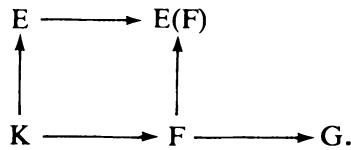
\includegraphics[keepaspectratio]{images/part001_e5f97af6.jpg}}\\
FIG. 2.

The condition is necessary: suppose that E and G are linearly disjoint over K. The same then holds of E and F (Prop. 7); on the other hand, if B is a basis of E over K, this is also a basis of the algebra F{[}E{]} over F; since B is by hypothesis free over G, F{[}E{]} and G are linearly disjoint over F, and the same is true of E(F) = F(E) and G, by Prop. 6.

The condition is sufficient: with the same notation it implies that B is free over F, hence it is a basis of F{[}E{]} over F; since F{[}E{]} and G are by hypothesis linearly disjoint over F, B is free over G, and this shows that E and G are linearly disjoint over K.

